\documentclass[tikz,border=3pt]{standalone}
\usetikzlibrary{calc}
\usetikzlibrary{intersections,through}

\begin{document}
    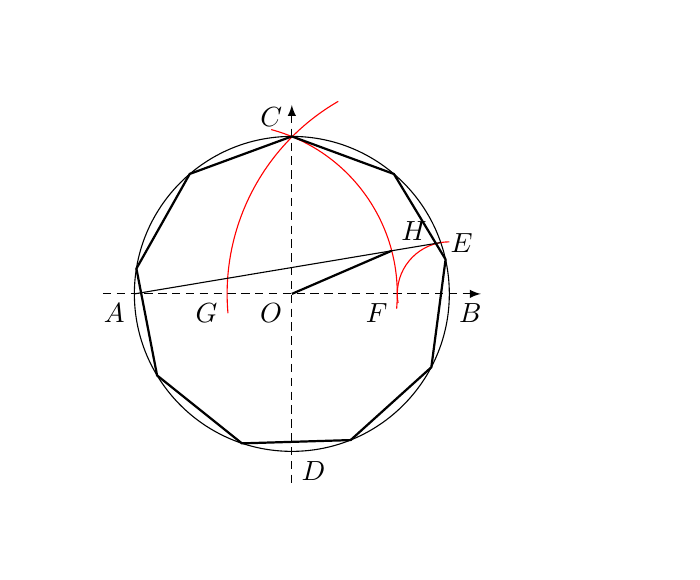
\begin{tikzpicture}[]
        % 标记点A,B,C,D,O
        \coordinate [label=below left:$A$] (A) at (0,0);
        \coordinate [label=below right:$B$] (B) at (4,0);
        \coordinate [label=above left:$C$] (C) at (2,2);
        \coordinate [label=below right:$D$] (D) at (2,-2);
        \coordinate [label=below left:$O$] (O) at (2,0);
        % 圆o
        \draw [name path=o] (O) circle (2);
        % AB, CD为圆的垂直中心线
        \draw [densely dashed,-latex,name path=AB] ($(A)!-.1!(B)$) -- ($(A)!1.1!(B)$);
        \draw [densely dashed,latex-,name path=CD] ($(C)!-.1!(D)$) -- ($(C)!1.1!(D)$);
        % 以B为圆心, BC为半径
        \path [name path=oCG]
        let 
            \p1=($(B)-(C)$),
            \n1={veclen(\x1,\y1)}
        in 
            (B) circle (\n1);
        % 标记圆弧与AB的交点G
        \path [name intersections={of=oCG and AB}]
            coordinate [label=below left:$G$] (G) at (intersection-1);
        % 绘制弧段
        \draw [red]
        let 
            \p1=($(B)-(C)$),
            \n1={veclen(\x1,\y1)}
        in 
            (G) arc (180:120:\n1)
            (G) arc (180:185:\n1);

        % 以G为圆心, GC为半径
        \path [name path=oCF]
        let 
            \p1=($(G)-(C)$),
            \n1={veclen(\x1,\y1)}
        in 
            (G) circle (\n1);
        \path [name intersections={of=AB and oCF}]
            coordinate [label=below left:$F$] (F) at (intersection-1);
        \draw [red] 
        let 
            \p1=($(G)-(C)$),
            \n1={veclen(\x1,\y1)}
        in 
            (F) arc (0:75:\n1)
            (F) arc (0:-5:\n1);

        % 以B为圆心, BF为半径
        \path [name path=oEF]
        let 
            \p1=($(B)-(F)$),
            \n1={veclen(\x1,\y1)}
        in 
            (B) circle (\n1);
        \path [name intersections={of=o and oEF}]
            coordinate [label=right:$E$] (E) at (intersection-1);
        \draw [red] 
        let 
            \p1=($(B)-(F)$),
            \n1={veclen(\x1,\y1)}
        in 
            (F) arc (180:90:\n1)
            (F) arc (180:190:\n1);

        % 连接AE交圆弧CF
        \draw [name path=AE] (A) -- (E);
        \path [name intersections={of=oCF and AE}]
            coordinate [label=above right:$H$] (H) at (intersection-1);
        % 连接OH
        \draw [thick] (O) -- (H);

        % 找到其他点
        \path [name path=o2]
        let
            \p2=($ (O) - (H) $),
            \n2={veclen(\x2,\y2)}
        in 
            (C) circle (\n2);
        \path [name intersections={of=o2 and o}]
            coordinate [] (C1) at (intersection-1)
            coordinate [] (C8) at (intersection-2);

        \path [name path=o3]
        let
            \p2=($ (O) - (H) $),
            \n2={veclen(\x2,\y2)}
        in 
            (C1) circle (\n2);
        \path [name intersections={of=o3 and o}]
            coordinate [] (C2) at (intersection-2);

        \path [name path=o4]
        let
            \p2=($ (O) - (H) $),
            \n2={veclen(\x2,\y2)}
        in 
            (C2) circle (\n2);
        \path [name intersections={of=o4 and o}]
            coordinate [] (C3) at (intersection-2);

        \path [name path=o5]
        let
            \p2=($ (O) - (H) $),
            \n2={veclen(\x2,\y2)}
        in 
            (C3) circle (\n2);
        \path [name intersections={of=o5 and o}]
            coordinate [] (C4) at (intersection-2);

        \path [name path=o6]
        let
            \p2=($ (O) - (H) $),
            \n2={veclen(\x2,\y2)}
        in 
            (C4) circle (\n2);
        \path [name intersections={of=o6 and o}]
            coordinate [] (C5) at (intersection-1);

        \path [name path=o7]
        let
            \p2=($ (O) - (H) $),
            \n2={veclen(\x2,\y2)}
        in 
            (C5) circle (\n2);
        \path [name intersections={of=o7 and o}]
            coordinate [] (C6) at (intersection-1);

        \path [name path=o8]
        let
            \p2=($ (O) - (H) $),
            \n2={veclen(\x2,\y2)}
        in 
            (C6) circle (\n2);
        \path [name intersections={of=o8 and o}]
            coordinate [] (C7) at (intersection-1);
        % 绘制正九边形
        \draw [thick] (C) -- (C1) -- (C2) -- (C3) -- (C4) -- (C5) -- (C6) -- (C7) -- (C8) -- cycle;
    \end{tikzpicture}
\end{document}